
\documentclass[twocolumn]{article}
\usepackage{hyperref}
\usepackage{enumitem}
\usepackage{graphicx}
\usepackage{amsmath}
\usepackage{mathpazo}
% \usepackage{multicol}
\usepackage[a4paper,
            bindingoffset=0.2in,
            left=1in,
            right=1in,
            top=1in,
            bottom=1in,
            footskip=.25in]{geometry}

\begin{document}
\title{MS Technical Paper: \\ Placement Algorithms for Heterogenous FPGAs}
\author{Brian B Cheng \\ Rutgers University Department of Electrical and Computer Engineering}


\date{}
\maketitle

\section{Keywords}
\begin{itemize}
    \item FPGA, EDA, Placement, Simulated Annealing, Optimization, RapidWright
\end{itemize}


\section{Abstract}
    fdsafdsafdsa.

\section{Introduction}

    Field-Programmable Gate Arrays (FPGAs) have witnessed rapid growth in capacity and versatility, driving significant advances in computer-aided design (CAD) and electronic design automation (EDA) methodologies. 
    Since the early-to-mid 2000s, the stagnation of single-processor performance relative to the rapid increase in integrated circuit sizes has led to a design productivity gap, where the computational effort for designing complex chips continues to rise. 
    In FPGA CAD flows—which traditionally encompass logic synthesis, placement, routing, and bitstream generation—the placement stage has emerged as one of the most time-consuming processes. 
    Inefficiencies in placement not only extend design times from hours to days, thereby elevating cost and reducing engineering productivity, but also limit the broader adoption of FPGAs by software engineers who expect compile times akin to those of conventional software compilers. 

    For these reasons, FPGA placement remains a critical research effort even today. 
    In this paper, we study and implement established placement methods by leveraging RapidWright, which is a semi-open-source API that offers backend access to Xilinx's industry-standard FPGA environment, Vivado. 
    We implement multiple variations of simulated annealing placers for Xilinx's 7-series FPGAs, with an emphasis on minimizing total wirelength while mitigating runtime. 
    Our implementation is organized into three consecutive substages. 
    The \textbf{prepacking} stage involves traversing a raw EDIF netlist to identify recurring cell patterns—such as CARRY chains, DSP cascades, and LUT-FF pairs—that are critical for efficient mapping and legalization. 
    In the subsequent \textbf{packing} stage, these identified patterns, along with any remaining loose cells, are consolidated into SiteInst objects that encapsulate the FPGA’s discrete resource constraints and architectural nuances. 
    Finally, the \textbf{placement} stage employs a simulated annealing (SA) algorithm to optimally assign SiteInst objects to physical sites, aiming to minimize total wirelength while adhering to the constraints of the 7-series architecture. 

    Simulated annealing iteratively swaps placement objects guided by a cost function that decides which swaps should be accepted or rejected. 
    Hill climbing is permitted by occasionally accepting moves that increase cost, in hope that such swaps may later lead to a better final solution. 
    SA remains a popular approach in FPGA placement research due to its simplicity and robustness in handling the discrete architectural constraints of FPGA devices. 
    While SA yields surprisingly good results given relatively simple rules, it is ultimately a heuristic and stochastic approach that explores the vast placement space by making random moves. 
    Most of these moves will be rejected, meaning that SA must run many iterations, usually hundreds to thousands, to arrive at a desirable solution. 

    In the ASIC domain, where placers must handle designs with millions of cells, the SA approach has largely been abandoned in favor of analytical techniques, owing to SA's runtime and poor scalability. 
    Modern FPGA placers have also followed suit, as new legalization strategies allow FPGA placers to leverage traditionally ASIC placement algorithms and adapt them to the discrete constraints of FPGA architectures. 
    While this paper does not present a working analytical placer, it will explore ways to build upon our existing infrastructure (prepacker and packer) to replace SA with AP. 

\section{A Brief History on FPGA Architecture}

    \begin{figure}
        \centering
        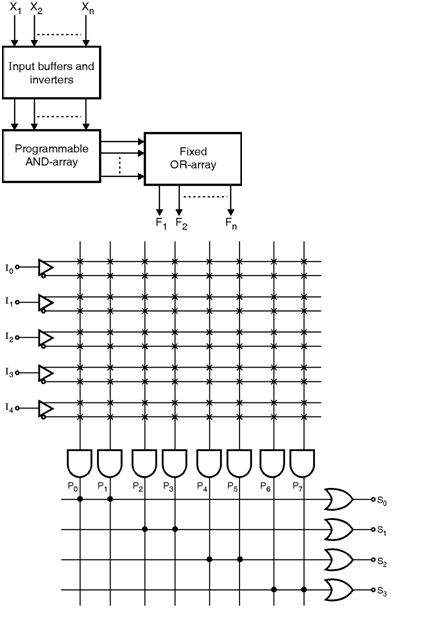
\includegraphics[width=8.5cm]{figures/pal_2.png}
        \caption{PAL architecture with 5 inputs, 8 programmable AND gates and 4 fixed OR gates}
        \label{fig:pla}
        % https://www.electronics-tutorial.net/Programmable-Logic-Device-Architectures/Programmable-Logic-Devices/Programmable-Array-Logic-PAL/
        % https://www.naukri.com/code360/library/difference-between-pla-and-pal 
    \end{figure}

    Before any work can begin on a placer, it is necessary to understand both the objects to be placed and the medium in which they are placed.

    Configurable logic devices have undergone significant evolution over the past four decades. 
    The journey began with the Programmable Logic Array (PLA) in the early 1970s. 
    The PLA implemented output logic using a programmable-OR and programmable-AND plane that formed a sum-of-products equation for each output through programmable fuses. 
    Around the same time, the Programmable Array Logic (PAL) was introduced. 
    The PAL simplified the PLA by fixing the OR gates, resulting in a fixed-OR, programmable-AND design, which sacrificed some logic flexibility to simplify its manufacture.

    \begin{figure}
        \centering
        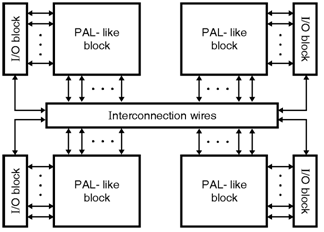
\includegraphics[width=7.5cm]{figures/cpld.png}
        \caption{CPLD architecture with 4 CLBs (PAL-like blocks)}
        \label{fig:cpld}
        % https://www.electronics-tutorial.net/Programmable-Logic-Device-Architectures/CPLD/Complex-Programmable-Logic-Device-CPLDs/
    \end{figure}

    Later in the same decade came the Complex Programmable Logic Device (CPLD), which took the form of an array of Configurable Logic Blocks (CLBs). 
    These CLBs were typically modified PAL blocks that included the PAL itself along with macrocells such as flip-flops, multiplexers, and tri-state buffers. 
    The CPLD functioned as an array of PALs connected by a programmable switch matrix and could be programmed using a hardware description language (HDL) like VHDL. 

    \begin{figure}
        \centering
        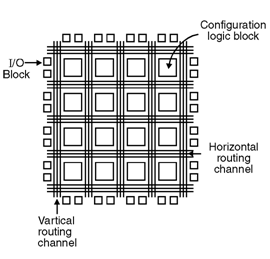
\includegraphics[width=7.0cm]{figures/fpga.png}
        \caption{Homogenous island-style FPGA architecture with 16 CLBs in a grid}
        \label{fig:fpga}
        % https://www.electronics-tutorial.net/Programmable-Logic-Device-Architectures/FPGA/Field-programmable-gate-array-FPGA/
    \end{figure}

    The mid-1980s saw the introduction of the homogeneous FPGA, which was built as a grid of CLBs. 
    Rather than using a central programmable switch matrix as in CPLDs, FPGAs adopted an island style architecture in which each CLB is surrounded on all sides by programmable routing resources. 
    The first commercially viable FPGA, produced by Xilinx in 1984, featured 16 CLBs arranged in a 4x4 grid. 
    As FPGA technology advanced, CLBs were redesigned to use lookup tables (LUTs) instead of PAL arrays for greater logic density. 
    The capacity of an FPGA was often measured by how many logical elements or CLBs it offered, which grew from hundreds to thousands and now to hundreds of thousands of CLBs.

    This brings us to modern day FPGA architectures.
    To meet the needs of increasingly complex designs, FPGA vendors introduced heterogeneous FPGAs. 
    In these devices, hard macros such as Block RAM (BRAM) and Digital Signal Processing (DSP) slices are integrated into the programmable logic fabric along with CLBs. 
    This design enables the direct instantiation of common subsystems like memories and multipliers, without having to implement them solely with CLBs. 
    Major vendors such as Xilinx and Altera now employ heterogeneous island-style architectures in their devices. 
    As designs become increasingly large and complex, FPGAs become increasingly heterogenous as they incorporate a wider variety of hard macros, including embedded CPUs and communications blocks, into the fabric.

\section{Xilinx 7-Series Architecture}

    \begin{figure*}
        \centering
        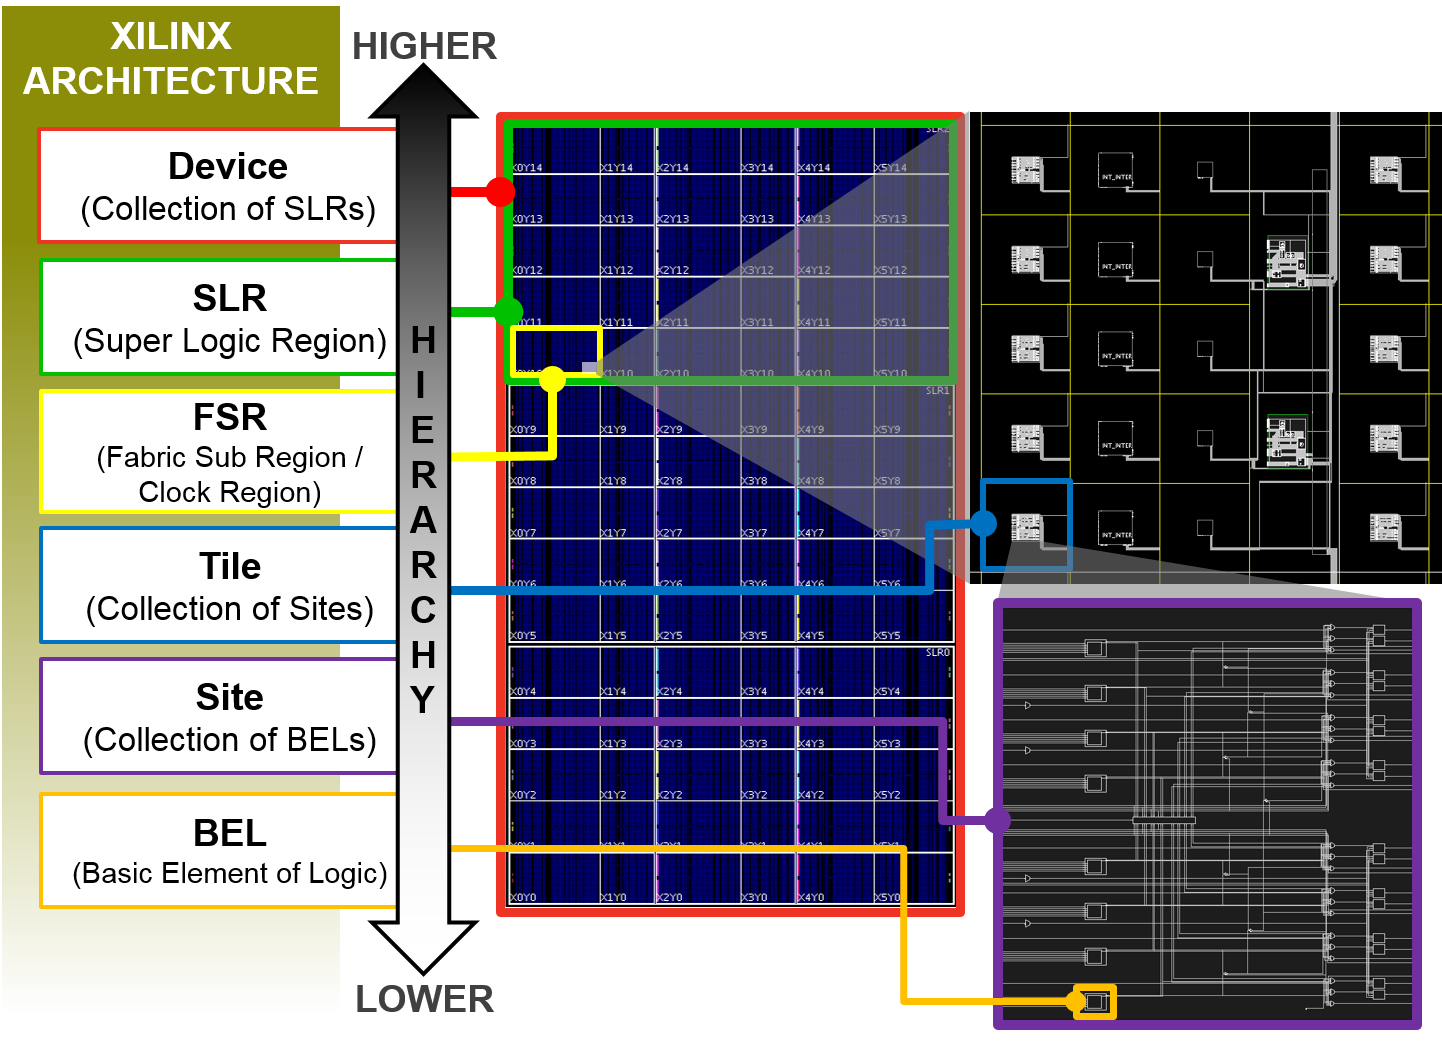
\includegraphics[width=\textwidth]{figures/hierarchy.png}
        \caption{Architecture Hierarchy of a Xilinx FPGA (Ultrascale)}
        \label{fig:hierarchy}
    \end{figure*}

    Xilinx introduced the 7-Series architecture in 2010 which followed the heterogeneous island-style architecture. 
    Then in 2013 Xilinx unveiled the Ultrascale architecture which made several improvements on the 7-Series architecture.
    Although the cutting edge of FPGAs follow the Ultrascale architecture, this paper focuses on the former 7-Series devices due to their greater accessibility for beginner users and compatibility with open source tooling.

    Figure~\ref{fig:hierarchy} illustrates the architectural hierarchy of an Ultrascale Xilinx FPGA. 
    The architecture hierarchy is the same for the 7-Series devices. 
    At its most basic level, an FPGA is a vast physical array of replicated atomic components known as Basic Elements of Logic (BELs). 
    These BELs, which include programmable lookup tables (LUTs), flip flops (FFs), and programmable interconnects, form the fundamental building blocks for custom digital circuit implementations on FPGAs. 

    In the FPGAs 7-Series FPGAs, additional BELs like Block RAM (BRAM) and Digital Processing Slices (DSPs) are also available, creating a more heterogeneous programmable logic fabric. 
    These dedicated resources allow designers to implement common digital structures, such as multipliers and memories, without having to recreate them from scratch using only LUTs and flip flops. 

    The Xilinx architectural hierarchy organizes these BELs into increasingly abstract structures. 
    \textbf{BELs} are packaged into \textbf{Sites}, which are then embedded into \textbf{Tiles}, which are subsequently consolidated into \textbf{Clock Regions}. 
    In high-end Xilinx devices, Clock Regions may be further consolidated into \textbf{Super Logic Regions} (SLRs). 
    However, for the scope of this paper, we focus on Xilinx devices that have only a single SLR. 

\section{The FPGA Design Flow and Toolchain}
    
    \begin{figure}
        \centering
        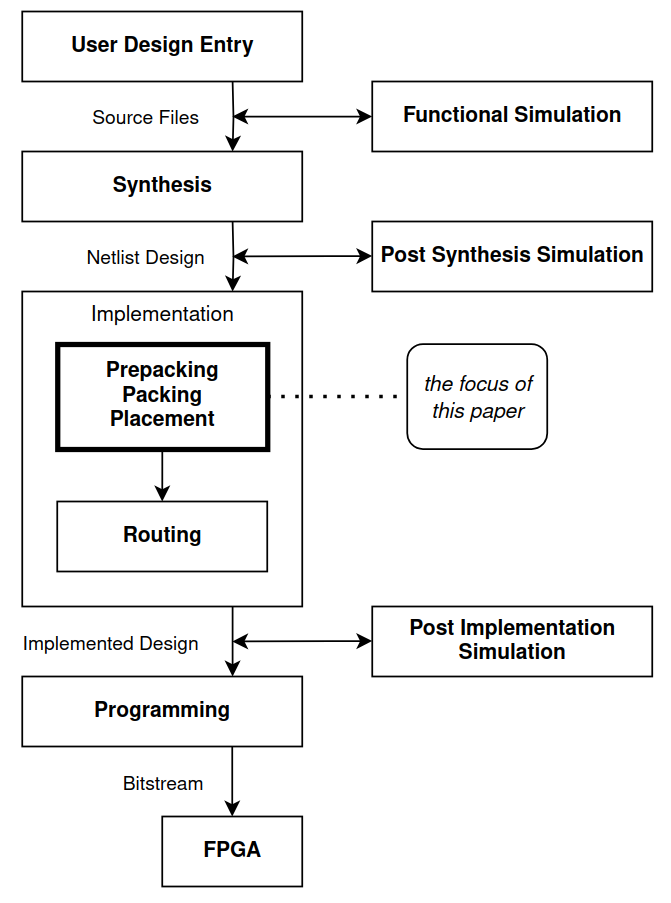
\includegraphics[width=7.0cm]{figures/design_flow.png}
        \caption{A typical FPGA design and verification flow}
        \label{fig:design_flow}
    \end{figure}

    Figure \ref{fig:design_flow} shows a typical FPGA design and verification flow.
    The FPGA design flow takes a high-level digital design written in an HDL and generates a configuration file that programs the physical FPGA. 

    The process begins with \textbf{design entry}, where an engineer describes the functionality of their circuit using a hardware description language (HDL) such as Verilog or VHDL. This description abstracts away details of the physical hardware while defining the logic and behavior of the design.

    Next, the \textbf{synthesis} tool interprets the HDL code and generates a netlist that represents the design in terms of basic logic elements, such as lookup tables (LUTs) and flip flops. 
    During this stage, substages like instantiation, substitution, inference, optimization, and technology mapping are applied to map the user design to a particular FPGA architecture.

    After synthesis, the \textbf{placement} tool assigns each logic element in the netlist a specific location within the FPGA’s fabric. 
    This stage can include substages of prepacking, packing, global placement, legalization, and detailed placement. 
    The objective is to place the logical cell instances of the netlist onto physical BELs on the device in a way that minimizes delay, satisfies design constraints, and simplifies routing. 

    Following placement, the \textbf{routing} tool connects the placed elements by assigning physical wiring resources to the nets in the netlist. 
    The router determines their paths through the programmable interconnect network while attempting to meet timing and performance constraints.
    
    Placement and routing are generally referred to together as the \textbf{implementation} stage, as both stages are interdependent and must adhere to the constraints of the same device.
    State of the art (SOTA) tools will perform routing-aware placement for greater optimization.

    The final stage is the \textbf{bitstream} generation, where a vendor-specific programming tool produces a configuration file or bitstream that programs the physical FPGA device. 
    The bitstream specifies the state of every configurable element—logic blocks, routing switches, and hard macros—ensuring the FPGA implements the user's design.

    Throughout the flow, additional tools, such as constraint managers and timing analyzers, are used to enforce design rules and verify that the implementation meets required performance specifications. 

    Parallel to this entire design flow are simulators for which the user can write testbenches to verify their design at different stages of implementation.
    Xilinx's Vivado, for example, provides functional simulation, post-implementation simulation, and post-implementation timing simulation.

    This integrated toolchain, whether provided by FPGA vendors or open source communities, facilitates the transformation from an abstract HDL description to a functioning hardware configuration.


\section{RapidWright API}
    \begin{figure}
        \centering
        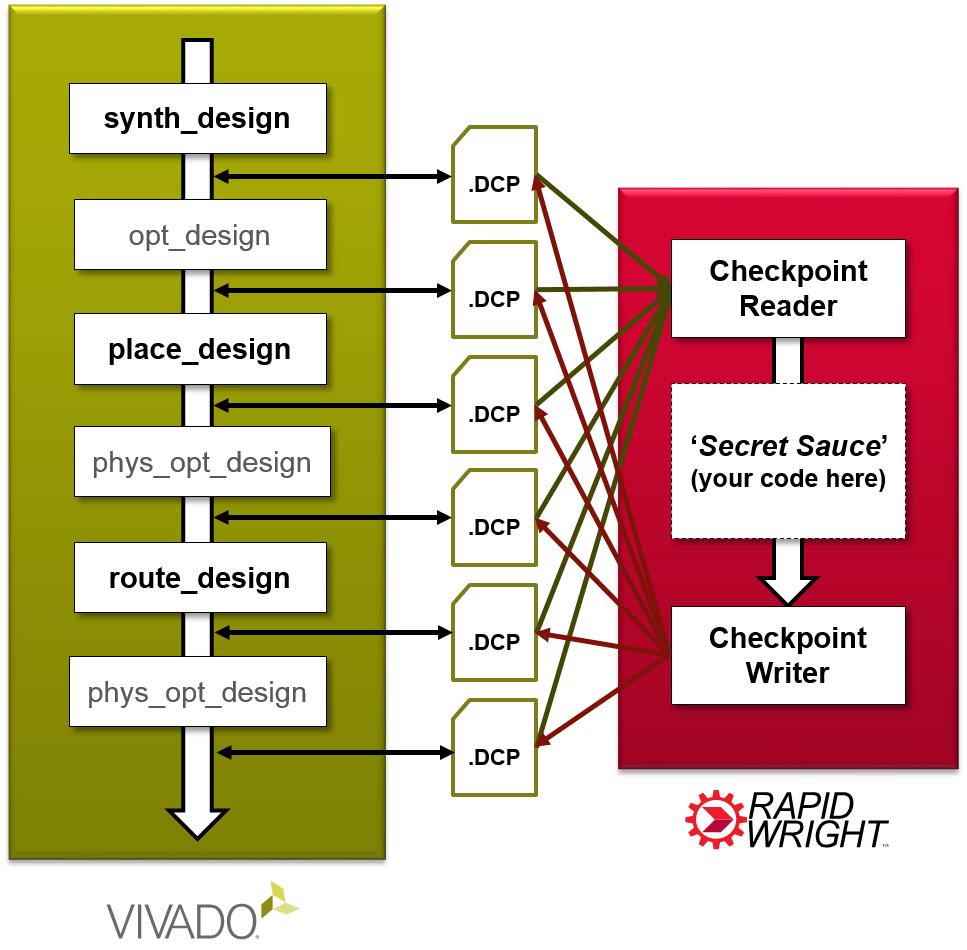
\includegraphics[width=6.5cm]{figures/vivado_dcps.png}
        \caption{Showing how RapidWright can take a design checkpoint at different stages of the Vivado toolchain, make customizations, then feed it back into the toolchain.}
        \label{fig:device_carry_chain_routing}
    \end{figure}

    DO WE REALLY NEED THIS SECTION? JUST REFERENCE THE RW DOCUMENTATION.

    The RapidWright API offers a user-friendly toolkit to take pre-implemented designs, that is, designs that have already been placed and/or routed by Vivado, and make custom optimizations to fit complex design criteria. 
    RapidWright has several "BlockPlacers", a general Router, but no general Placer. 
    We use this API to implement a crude general placer, in our case, a simulated annealer. 
    (Show what parts of the FPGA toolchain that RapidWright already has and how our placer fits into that toolchain). 

    There are three packages of objects that are most relavent to building our placer: the edif package, design package, and device package. 

    \subsection{Device Objects}
    The \textbf{device} package contains the classes that correspond to constructs in the hardware and/or silicon devices. 
    The most prominent class, aptly named Device, represents a specific product family member (like the xc7z020 device of the 7-series family) and provides a reference to all of the logical and routing resources available on the device. 
    There device classes can be separated into two groups: logical and routing. 
    Among the logical classes are the BEL, Site, Tile, and ClockRegion objects discussed before. 
    Among the routing classes are BELPin, SitePin, PIP (programmable interconnect point), Wire, and Node. 

    \subsection{Design Package}
    The \textbf{design} package is the collection of objects used to describe how a logical netlist maps to the device netlist. 
    The design is also referred to as the "physical netlist" or "implementation". 
    It contains all of the primitive logical cell mappings to hardware, specifically the cells to BEL placements and physical net mapping to programmable interconnect or routing. 

    \subsection{EDIF Package}
    In Vivado, all designs post synthesis have a logical netlist that can be exported in the Electronic Design Interchange Format (EDIF) netlist format. 
    The synthesis stage of the FPGA toolchain produces an EDIF file, which is a low-level file containing the technology-mapped netlist. 
    The EDIFNetlist is the top level class that contains the netlist and cell libraries. 
    The EDIFNetlist keeps a reference to the top cell which is wrapped in the EDIFDesign class. 
    It also maintains a top cell instance reference that is generated when the file is loaded. 


\section{Placement Implementation}
    (Describe the algorithm, then in context of 7-Series arhictecture). \\
    \subsection{PrePacking}
        In the prepacking stage, we traverse the raw EDIF Netlist to identify recurring cell patterns. In particular, we will specifically look for CARRY chains, DSP cascades, and LUT-FF pairs.
        \subsection{CARRY Chains}
            Each SLICE Site contains one CARRY4 BEL.
            Each CLB Tile contains two SLICE Sites.
            CARRY chains span vertically across multiple SLICE Sites/Tiles. (Show picture)
            \begin{figure}
                \centering
                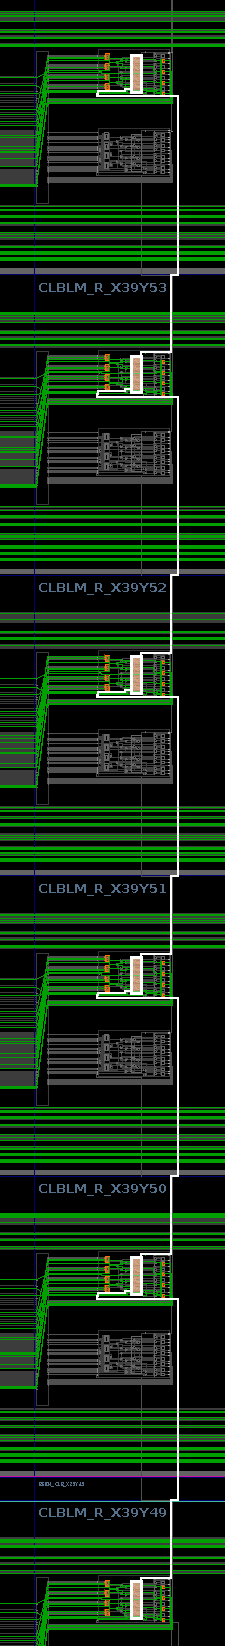
\includegraphics[width=3.0cm]{figures/carry_chain_routes.png}
                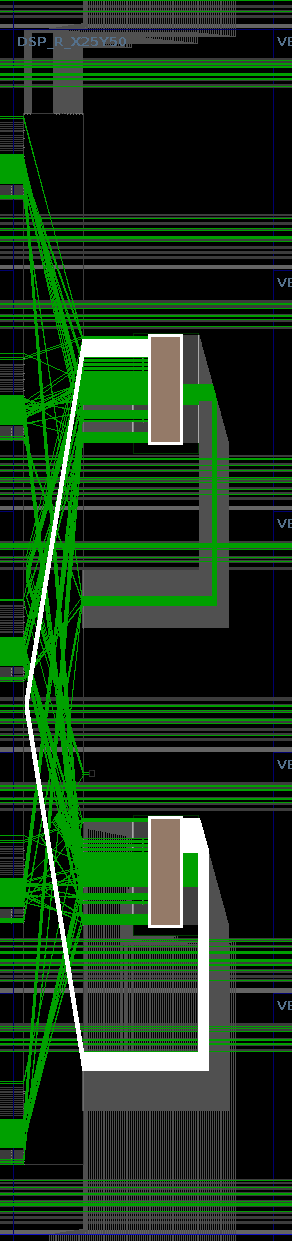
\includegraphics[width=3.0cm]{figures/dsp_cascade_routes.png}
                \caption{A Carry Chain of length 6 spanning 6 Tiles. On the left, the cell-only representation. On the right, cells with routing representation.}
                \label{fig:device_carry_chain_routing}
            \end{figure}
        \subsection{DSP Cascades}
            Each DSP Site contains one DSP BEL.
            Each DSP Tile contains two DSP Sites.
            DSP chains can span vertically across multiple DSP Sites/Tiles.

        \subsection{LUT-FF Pairs}
            Identify unique CE-SR net pairs. All FF cells in a Site must share the same CE and SR nets.
    \subsection{Packing}
        In the packing stage, we take the identified cell clusters and pack them into SiteInst Design objects which target the Device Site objects.
        \subsection{CLB Sites}
            Can support LUT-FF pairs, loose LUTs, loose FFs, CARRY chains.
            Each SLICE has 8 "lanes" of LUT-FFs. 4 LUT5s and 4 LUT6s. 8 FFs.
            For SLICEMs, LUT6s can be configured as shallow 32-bit LUTRAMs or "RAMS32".
    \subsection{Placement}
        Create BEL "fields": CLB, DSP, CLB and DSP Chains, RAMs

        \subsection{Detailed Placement}







\section{Analytical Placement}
    Introduce placement with legalization methods. \\
    Many AP approaches use a Global placement, Legalization, then Detailed placement approach. \\
    Our SA only considers legal moves via bookkeeping structures, so it has no concept of global placement or legalization. \\
    It is a detailed placement only approach. \\
    \begin{itemize}
        \item Talk about HeAP as an example.
        \item Global Placement, Legalization, then Detailed Placement approach.
        \item Global placement using the Bound2Bound net model from SimPL.
        \item Legalization Step 1: \\
            Find an area of the device that is overutilized (illegal) for twhich the blocks contained within must spread to a larger area. \\
            To obtain this overutilized area, adjacent locations (Sites, Tiles, etc.) on the device that are occupied by more than one block (SiteInst, ModuleInst, etc.) are repeatedly clustered together, until all clusters are bordered on all sides by non-overutilized locations. \\ 
            Then, the area (?) is expanded in both the x and y dimensions (?) until it is large enough to accommodate all blocks contained within. \\
            Specifically, the area is expanded until its "occupance" \(O_A\) divided by its "capacity" \(C_A\) is less than a maximum "utilization factor" $\beta$, where $\beta$ is less than or equal to 1. HeAP uses 0.9.
        \item Legalization Step 2: \\
            Two cuts are generated: a "source cut" and a "target cut". \\
            The source cut pertains to the blocks being placed (SiteInsts in home buffer). \\ 
            The target cut pertains to the area into which the blocks are placed (away buffer). \\
            The source cut splits the blocks into 2 partitions, while the target cut splits the area into 2 sub-areas, into which the blocks in each partition are spread. \\
            Two objectives are minimized during this process: The imbalance between the number of blocks in each partition, and the difference in the utilization of each sub-area. \\
            Utilization defined as the occupancy divided by the capacity of the sub-area. \\
            \(U_{sub-area} = \frac{O_{sub-area}}{C_{sub-area}}\) \\
            To generate the source cut, the cells are first sorted by their x or y location, depending on the orientation of the desired cut. \\
            Once the cells are sorted, the source cut generation is akin to choosing a pivot in a sorted list, where all blocks to the left of the pivot are assigned to the left/bottom partition and all blocks to the right of the pivot are assigned to the right/top partition. \\
            The target cut is an x or y cut of the area such that all blocks in each partition fit in their respective sub-areas, and such that \( | U_{sub-area_1} 
             - U_{sub-area_2} | \) is minimized.




    \end{itemize}





\end{document}
